\subsection{Расчет потребления памяти iOS-клиентом}
\label{sec:eng:memory}

Для расчета потребления памяти iOS-клиентом будут использоваться стандартные инструменты Apple: \textit{Instruments} и \textit{Xcode}. В рамках данного ДП будет рассмотрено потребление памяти в трёх состояних клиента и оценён отпечаток в памяти экрана настроек.

Первым рассматриваемым состоянием является экран выбора адреса сервера. К моменту показа этого экрана большая часть приложения всё ещё не загружена и память потребляется в основном сторонними библиотеками и общими ресурсами. На рисурке \ref{sec:eng:memory:initial} отображена статистика потребления памяти на начальном экране, генерируемая \textit{Xcode}.

\begin{figure}[h]
  \centering
    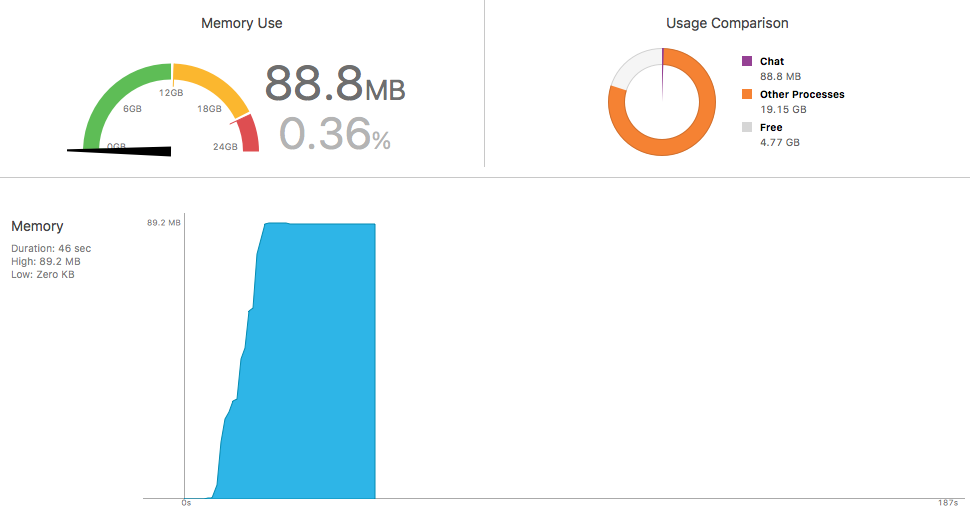
\includegraphics[width=1\textwidth]{inc/img/memory_initial.png}
  \caption{Потребление памяти iOS-клиентом на начальном экране}
  \label{sec:eng:memory:initial}
\end{figure}

На рисунке \ref{sec:eng:memory:used} отражено количество потребляемой памяти после полной загрузки приложения и показа экрана со списком всех диалогов. Как можно заметить, общий отпечаток в памяти вырос примерно на 30 мегабайт, что существенно меньше начального скачка, обусловленного загрузкой сторонних библиотек.

\begin{figure}[h]
  \centering
    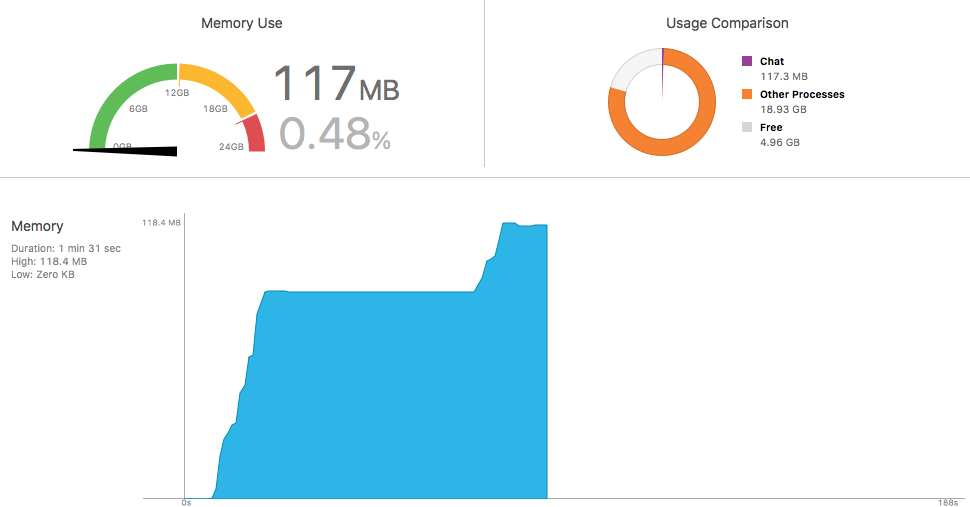
\includegraphics[width=1\textwidth]{inc/img/memory_used.png}
  \caption{Потребление памяти iOS-клиентом на экране списка диалогов}
  \label{sec:eng:memory:used}
\end{figure}

\textit{Xcode} хорошо подходит для беглого аудита потребления ресурсов клиентом, однако имеет ряд недостатков:

\begin{itemize}
	\item завышает значения в сравнении с потреблением ресурсов на настоящем устройстве;
	\item даёт малое количество информации;
	\item не даёт способов как-либо повлиять на алгоритм сбора данных, отфильтровать шумы.
\end{itemize}

Для серьёзного профилирования вместе с \textit{Xcode} поставляется приложение \textit{Instruments}, которое позволяет детально рассмотреть огромное количество метрик для клиентов под операционные системы Apple. В рамках данного дипломного проектирования, интересующим инструментов является монитор аллокаций, который позволяет:

\begin{itemize}
	\item отслеживать общее потребление памяти во времени;
	\item отслеживать изменение потребления памяти между определёнными событиями или произвольными моментами времени;
	\item просмотреть весь граф объектов, находящийся в данный момент в памяти или на стеке;
	\item проанализировать природу появления объекта и причины, по которым он не может освободить память;
	\item автоматически определять утечки памяти.
\end{itemize}

Для тестирования был выбран экран настроек приложения, на рисунке \ref{sec:eng:memory:generations} приведены результаты замеров, где:

\begin{explanation}
где & \textit{Generation A} & начальное поколение приложения, которое появляется в результате запуска; \\
    & \textit{Generation B} & поколение объектов, появившихся в результате показа экрана настроек; \\
    & \textit{Generation C} & поколение объектов, появившихся в результате закрытия экрана настроек; \\
    & \textit{Generation D} & поколение объектов, появившихся в результате повторного показа экрана настроек. \\
\end{explanation}

\begin{figure}[h]
  \centering
    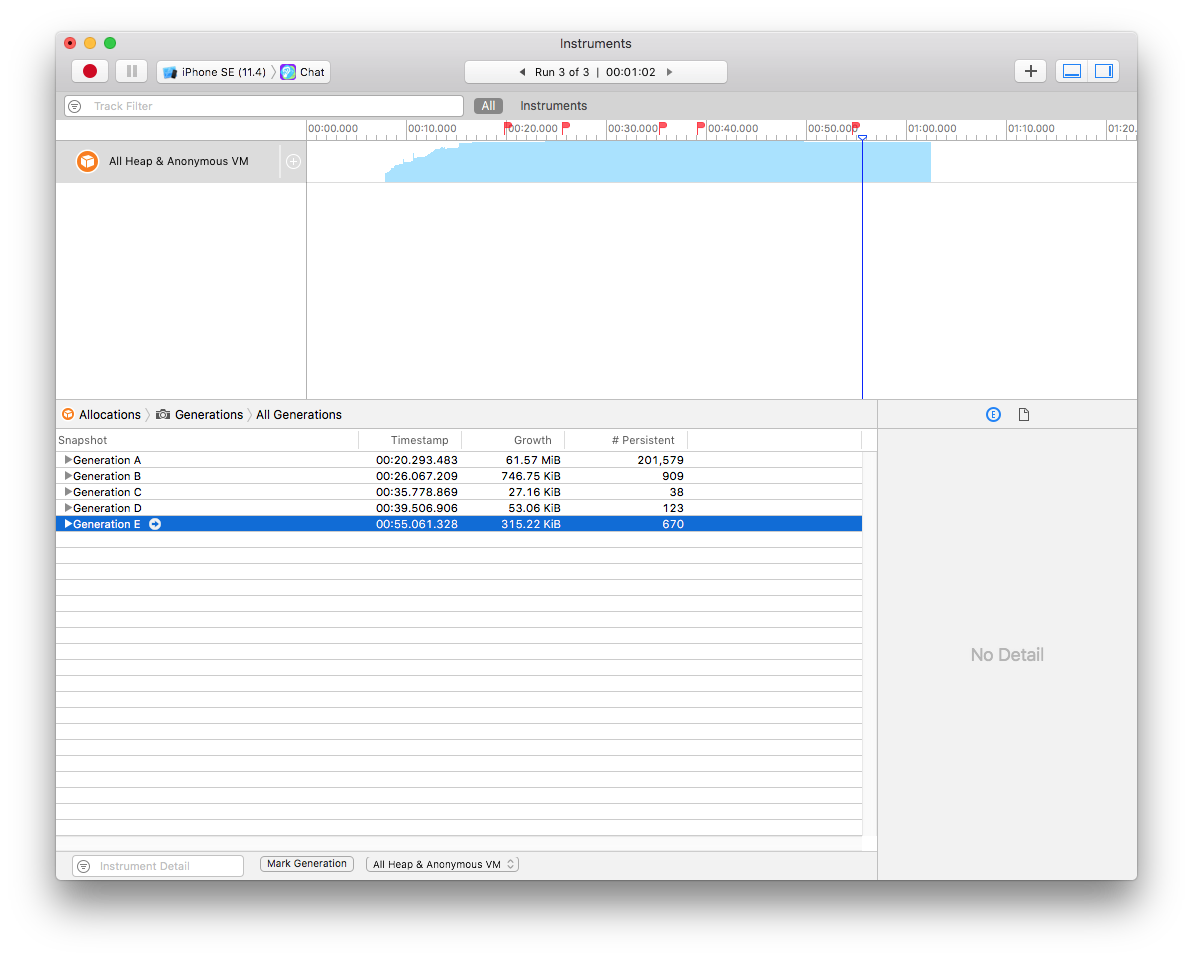
\includegraphics[width=1\textwidth]{inc/img/memory_generations.png}
  \caption{Потребление памяти iOS-клиентом в процессе работы с экраном настроек}
  \label{sec:eng:memory:generations}
\end{figure}

Как можно заметить, при закрытии экрана настроек не освобождается достаточное количество памяти, а при повторном открытии -- выделяется очень мало памяти. Это свидетельствует об утечки памяти, однако в данном случае частично утечка обусловлена наличием кэша на экране, который являтеся общим на приложении и очищается только при получении запроса от операционной системы. Основным потребителем памяти в приложении являются сторонние библиотеки, поэтому на этапе поддержки приложения будет произведён пересмотр используемх библиотек с возможной заменой или оптимизацией.